
\subsection{Polarización}

\par Se simularon los valores en reposo de los transistores de la etapa amplificadora clase G, junto con la máxima potencia disipada en cada uno. Los resultados se muestran en el cuadro ~\tableref{tab:PuntoQ_simulacion}:\\


\begin{table}[H]
    \setlength\arrayrulewidth{1pt}
    \arrayrulecolor{TABLEColor}
    \begin{center}
        \begin{tabular}{llllll}
        \hline\hline
            Transistor & $V_{BEQ}$ & $V_{CEQ}$ & $I_{CQ}$ & $P_{max}$\\
            \hline \hline
            Q1 (BC546C)     & 612mV     & 33.87V    & 549uA     & 18.6mW    \\
            Q2 (BC556B)     & -610mV    & -1.31V    & 549uA     & 722uW     \\
            Q3 (BC546B)     & 631mV     & 31.78V    & 1.1mA     & 35mW      \\
            Q4 (BC556B)     & -610mV    & 33.78V    & 549uA     & 334mW     \\
            Q5 (BC546B)     & 612mV     & 34.6V     & 549uA     & 19mW      \\
            Q6 (BC546B)     & 693mV     & 28.8V     & 9.71mA    & 280mW     \\
            Q7 (BC556B)     & -557mV    & 30V       & 170uA     & 5mW       \\
            Q8 (BC556B)     & -669mV    & 30.71V    & 9.57mA    & 294mW     \\ 
            Q9 (BD135)      & 676mV     & 2.96V     & 9.40mA    & 28mW      \\
            Q10(BD136)      & -722mV    & 13.9V     & 15mA      & 208mW     \\
            Q11(BD136)      & 10.95V    & 20.32V    & 31pA      & 1.1nW     \\
            Q12(BD135)      & -10.93V   & 20.32V    & 31pA      & 1.1nW     \\
            Q13(BD135)      & 693mV     & 13.88V    & 18.9mA    & 263mW     \\
            Q14(MJL21194)   & 1.04nV    & 20.32V    & 26pA      & 522pW     \\
            Q15(MJL21194)   & 722mV     & 14.6V     & 714mA     & 10.43W    \\
            Q16(MJL21193)   &-678mV     & 14.6V     & 718mA     & 10.49W    \\
            Q17(MJL21193)   &-986mV     & 20.32V    & 1.76pA    & 459pW     \\
            Q18(2N3906)     &-72mV      & 1.47V     & 1.47pA    & 2.2pW     \\
            Q19(2N3904)     &72mV       & 1.48V     &1.58pA     & 2.3pW     \\\hline\hline
        \end{tabular}
    \caption{Punto de reposo de los transistores y máxima potencia disipada en operación}
    \label{tab:PuntoQ_simulacion}
    \end{center}
\end{table}

\par En la figura ~\figref{fig:PuntoQ_simulacion} se pueden verificar los resultados de la simulación con las referencias en el circuito pertinente.

\begin{figure}[H]
    \centering
    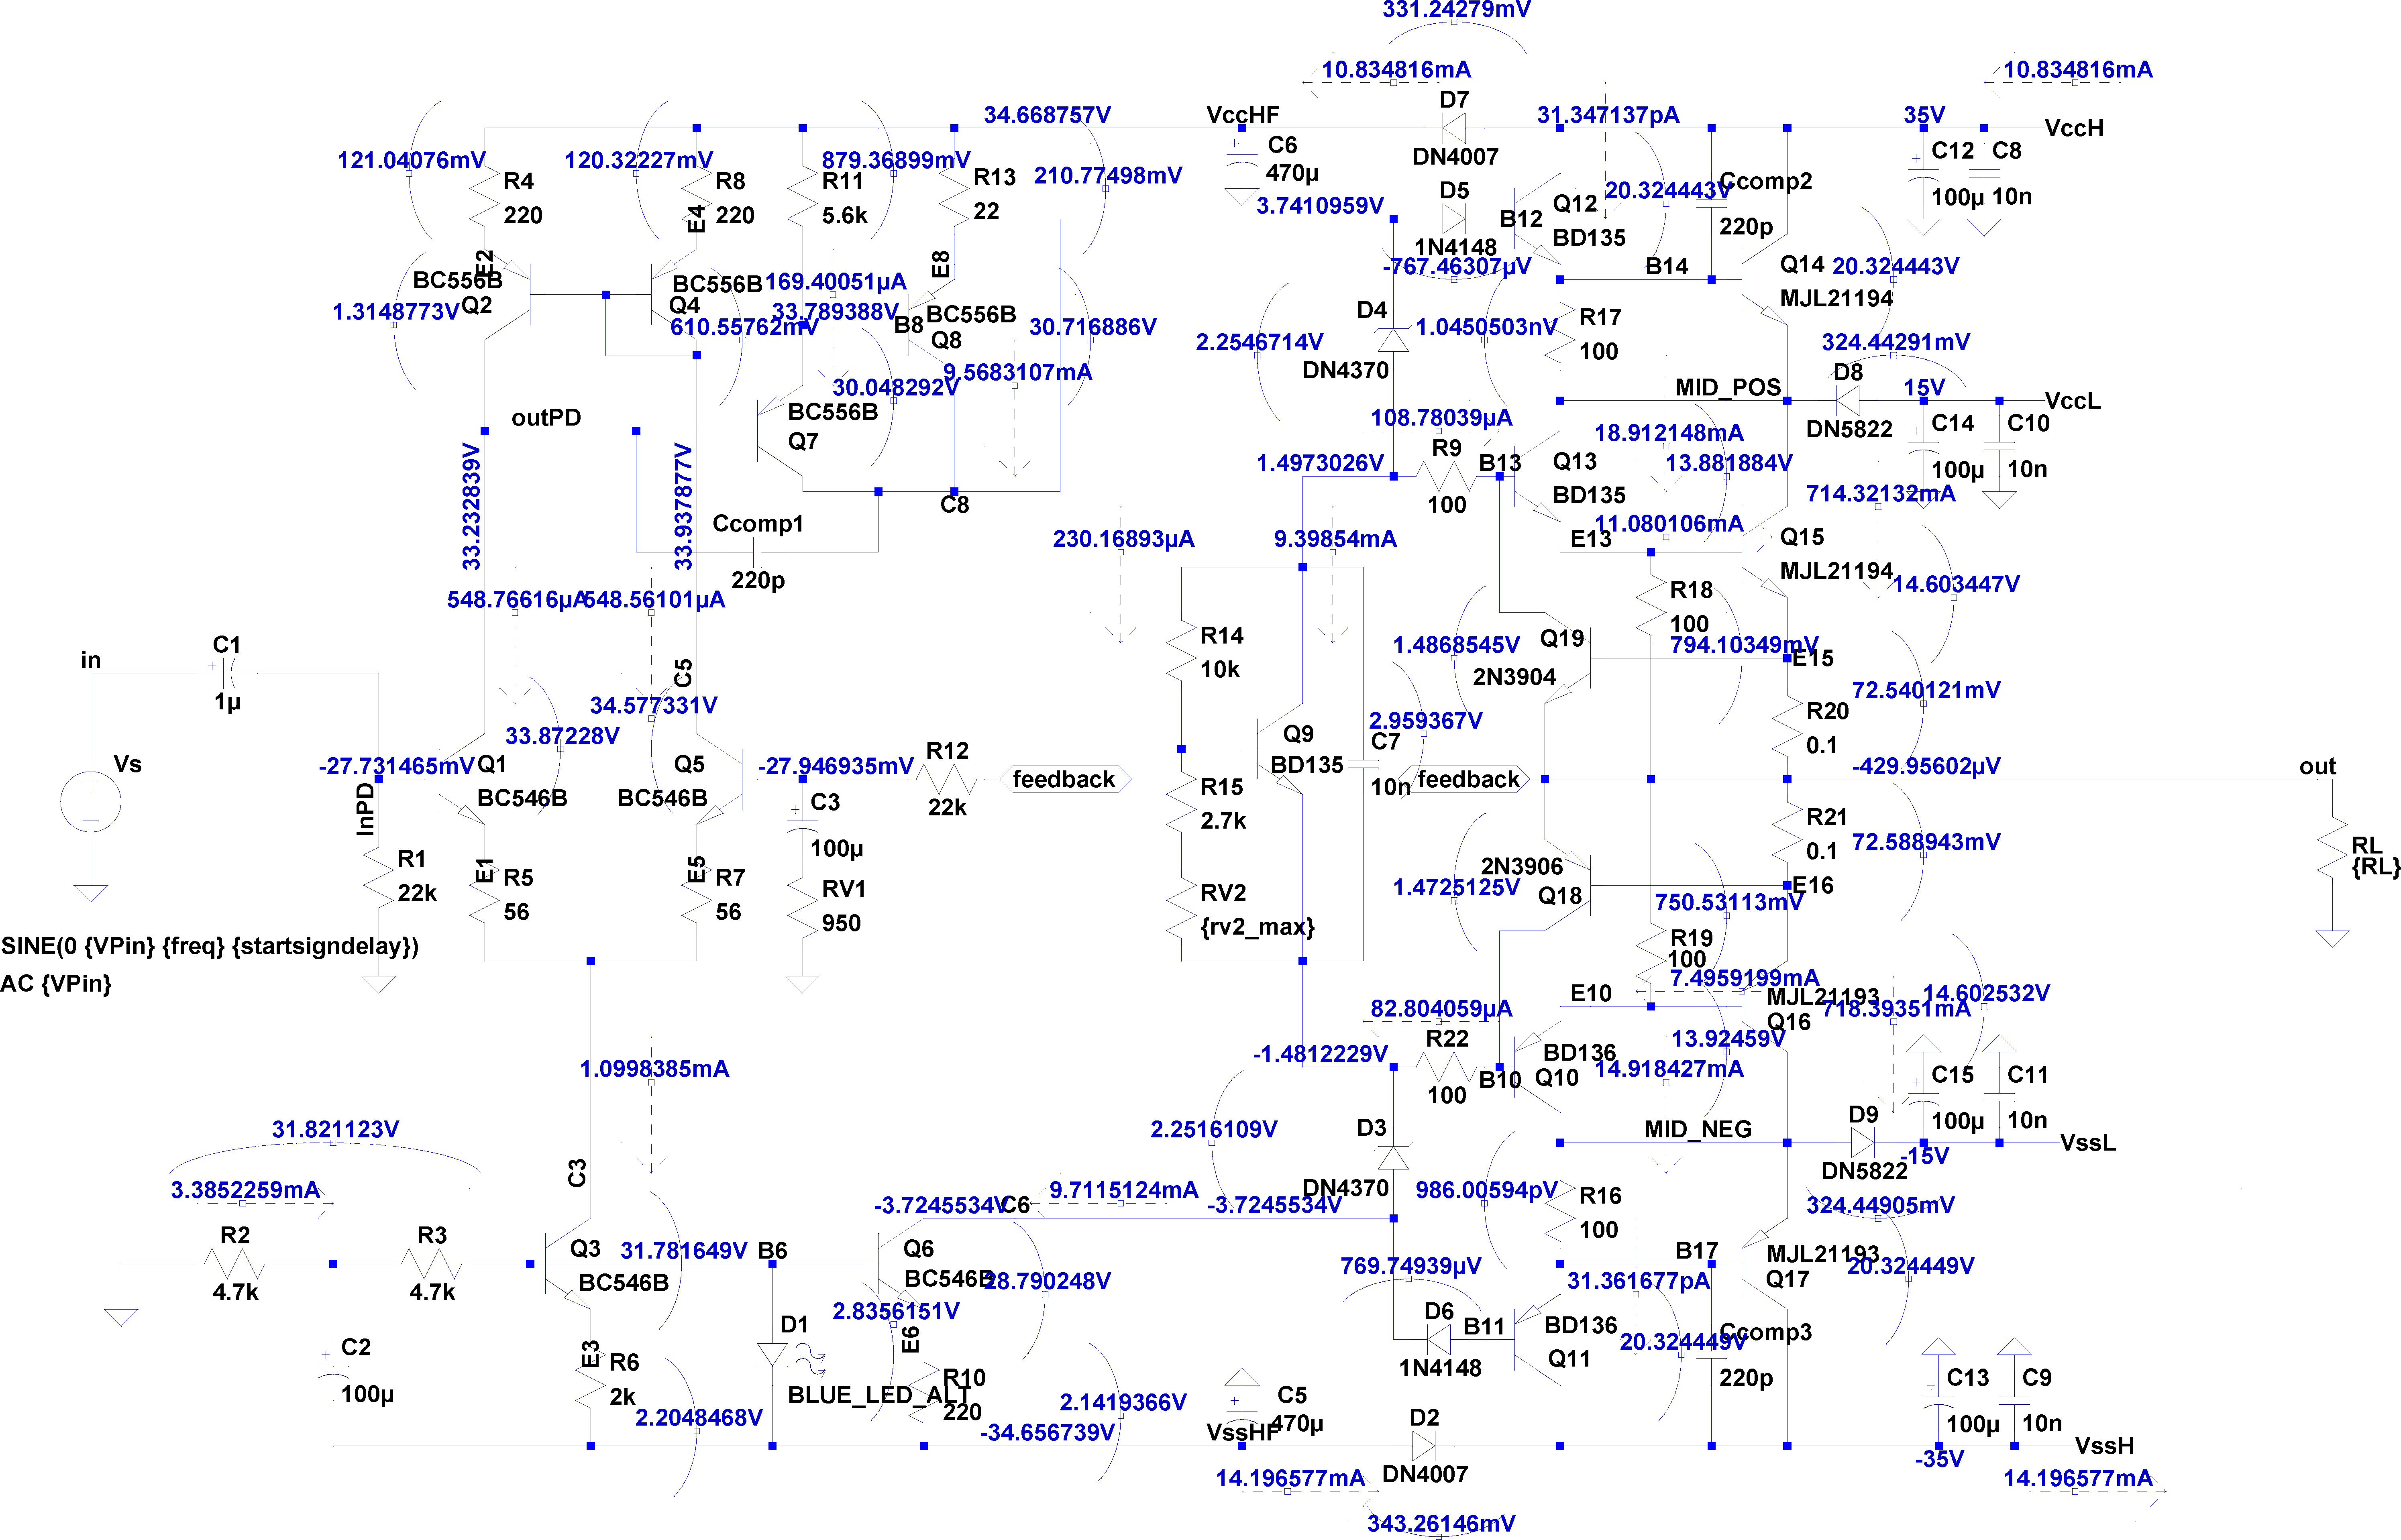
\includegraphics[scale=0.65]{./img/circuito/amplifier.png}
    \caption{Circuito simulado junto con los valores de polarización}
    \label{fig:PuntoQ_simulacion}
\end{figure}


\subsection{Simulación de ganancia de lazo}

\par En la figura ~\figref{fig:gain_loop_sim} se puede observar la ganancia de lazo del circuito, simulado a distintas frecuencias. A su vez, se especifica el margen de ganancia y de fase, para verificar la correcta estabilización del circuito. Obteniéndose de este modo:

\begin{itemize}
    \item Margen de ganancia: $29.21dB$
    \item Margen de fase: $86.12^\circ$
\end{itemize}

\begin{figure}[H]
    \centering
    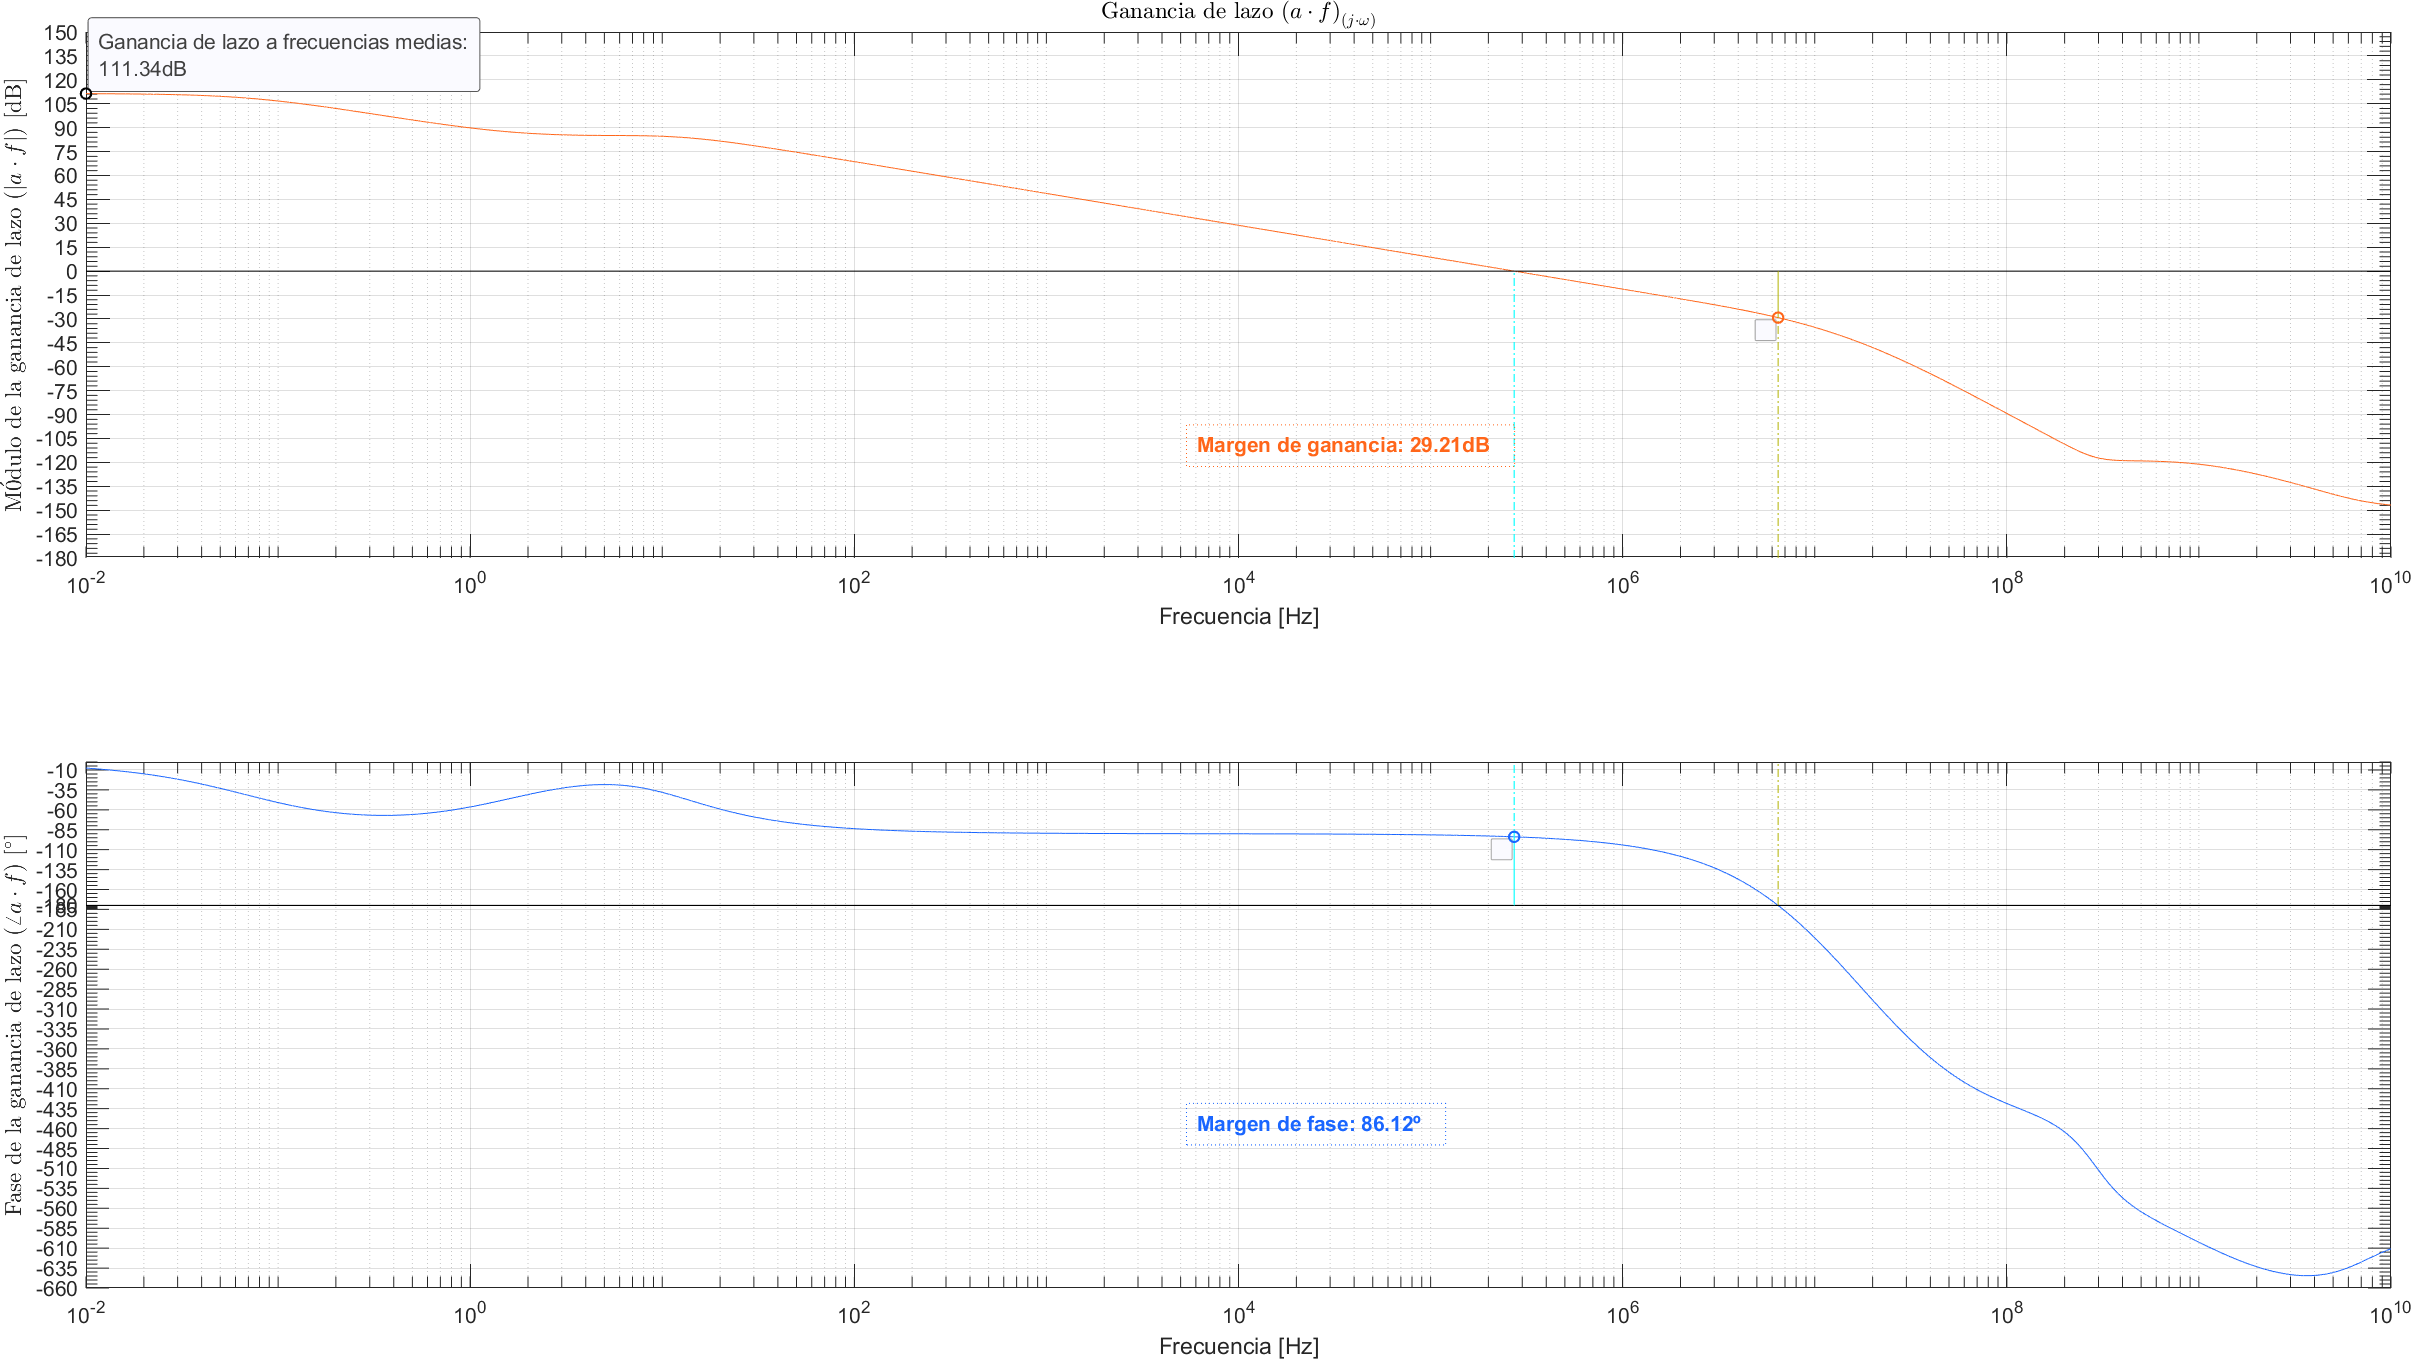
\includegraphics[scale=0.4]{./img/simulaciones/Loop/gain_loop.png}
    \caption{Ganancia de lazo simulado}
    \label{fig:gain_loop_sim}
\end{figure}


\subsection{Ancho de banda de potencia}

\par En la figura ~\figref{fig:Power_BW_sim}, se observa el resultado de la simulación del ancho de banda de potencia simulado.
\par Obtenemos en el circuito un ancho de banda de potencia de $97.89kHz$ con frecuencias de corte:

\begin{itemize}
    \item $f_l = 22.34Hz$
    \item $f_h = 97.84kHz$
\end{itemize}

\begin{figure}[H]
    \centering
    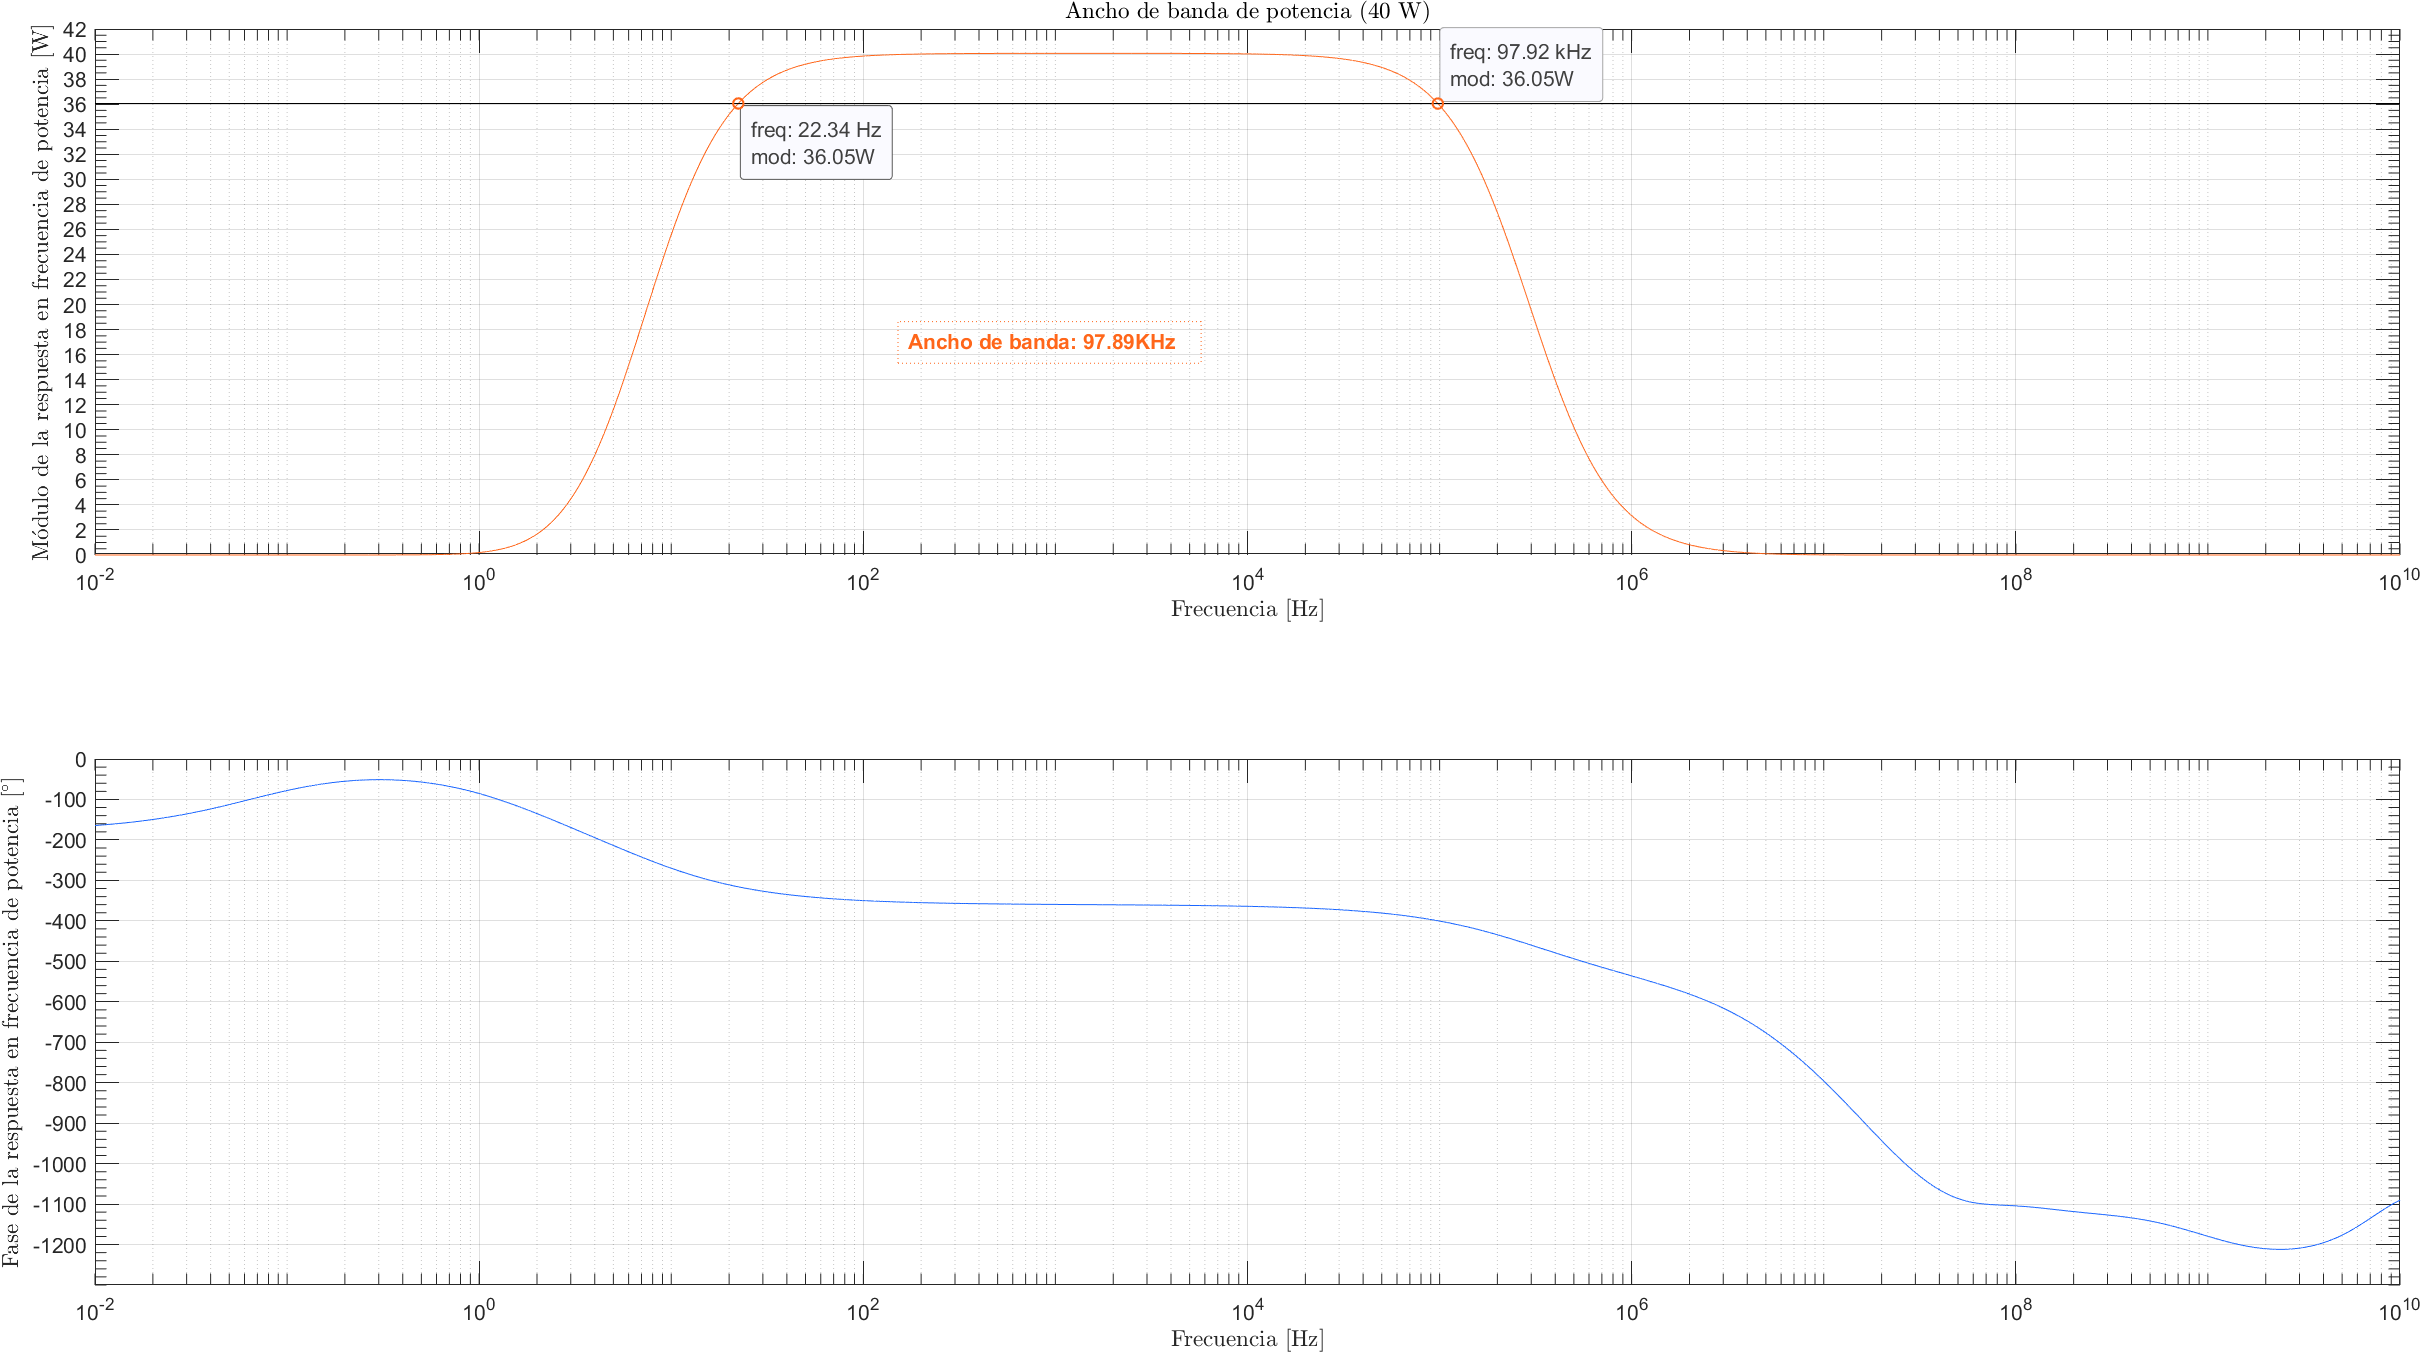
\includegraphics[scale=0.4]{./img/simulaciones/BW/Power_BW.png}
    \caption{Ancho de banda de potencia simulado}
    \label{fig:Power_BW_sim}
\end{figure}


\subsection{Impedancias de entrada y salida}

\begin{figure}[H]
    \centering
    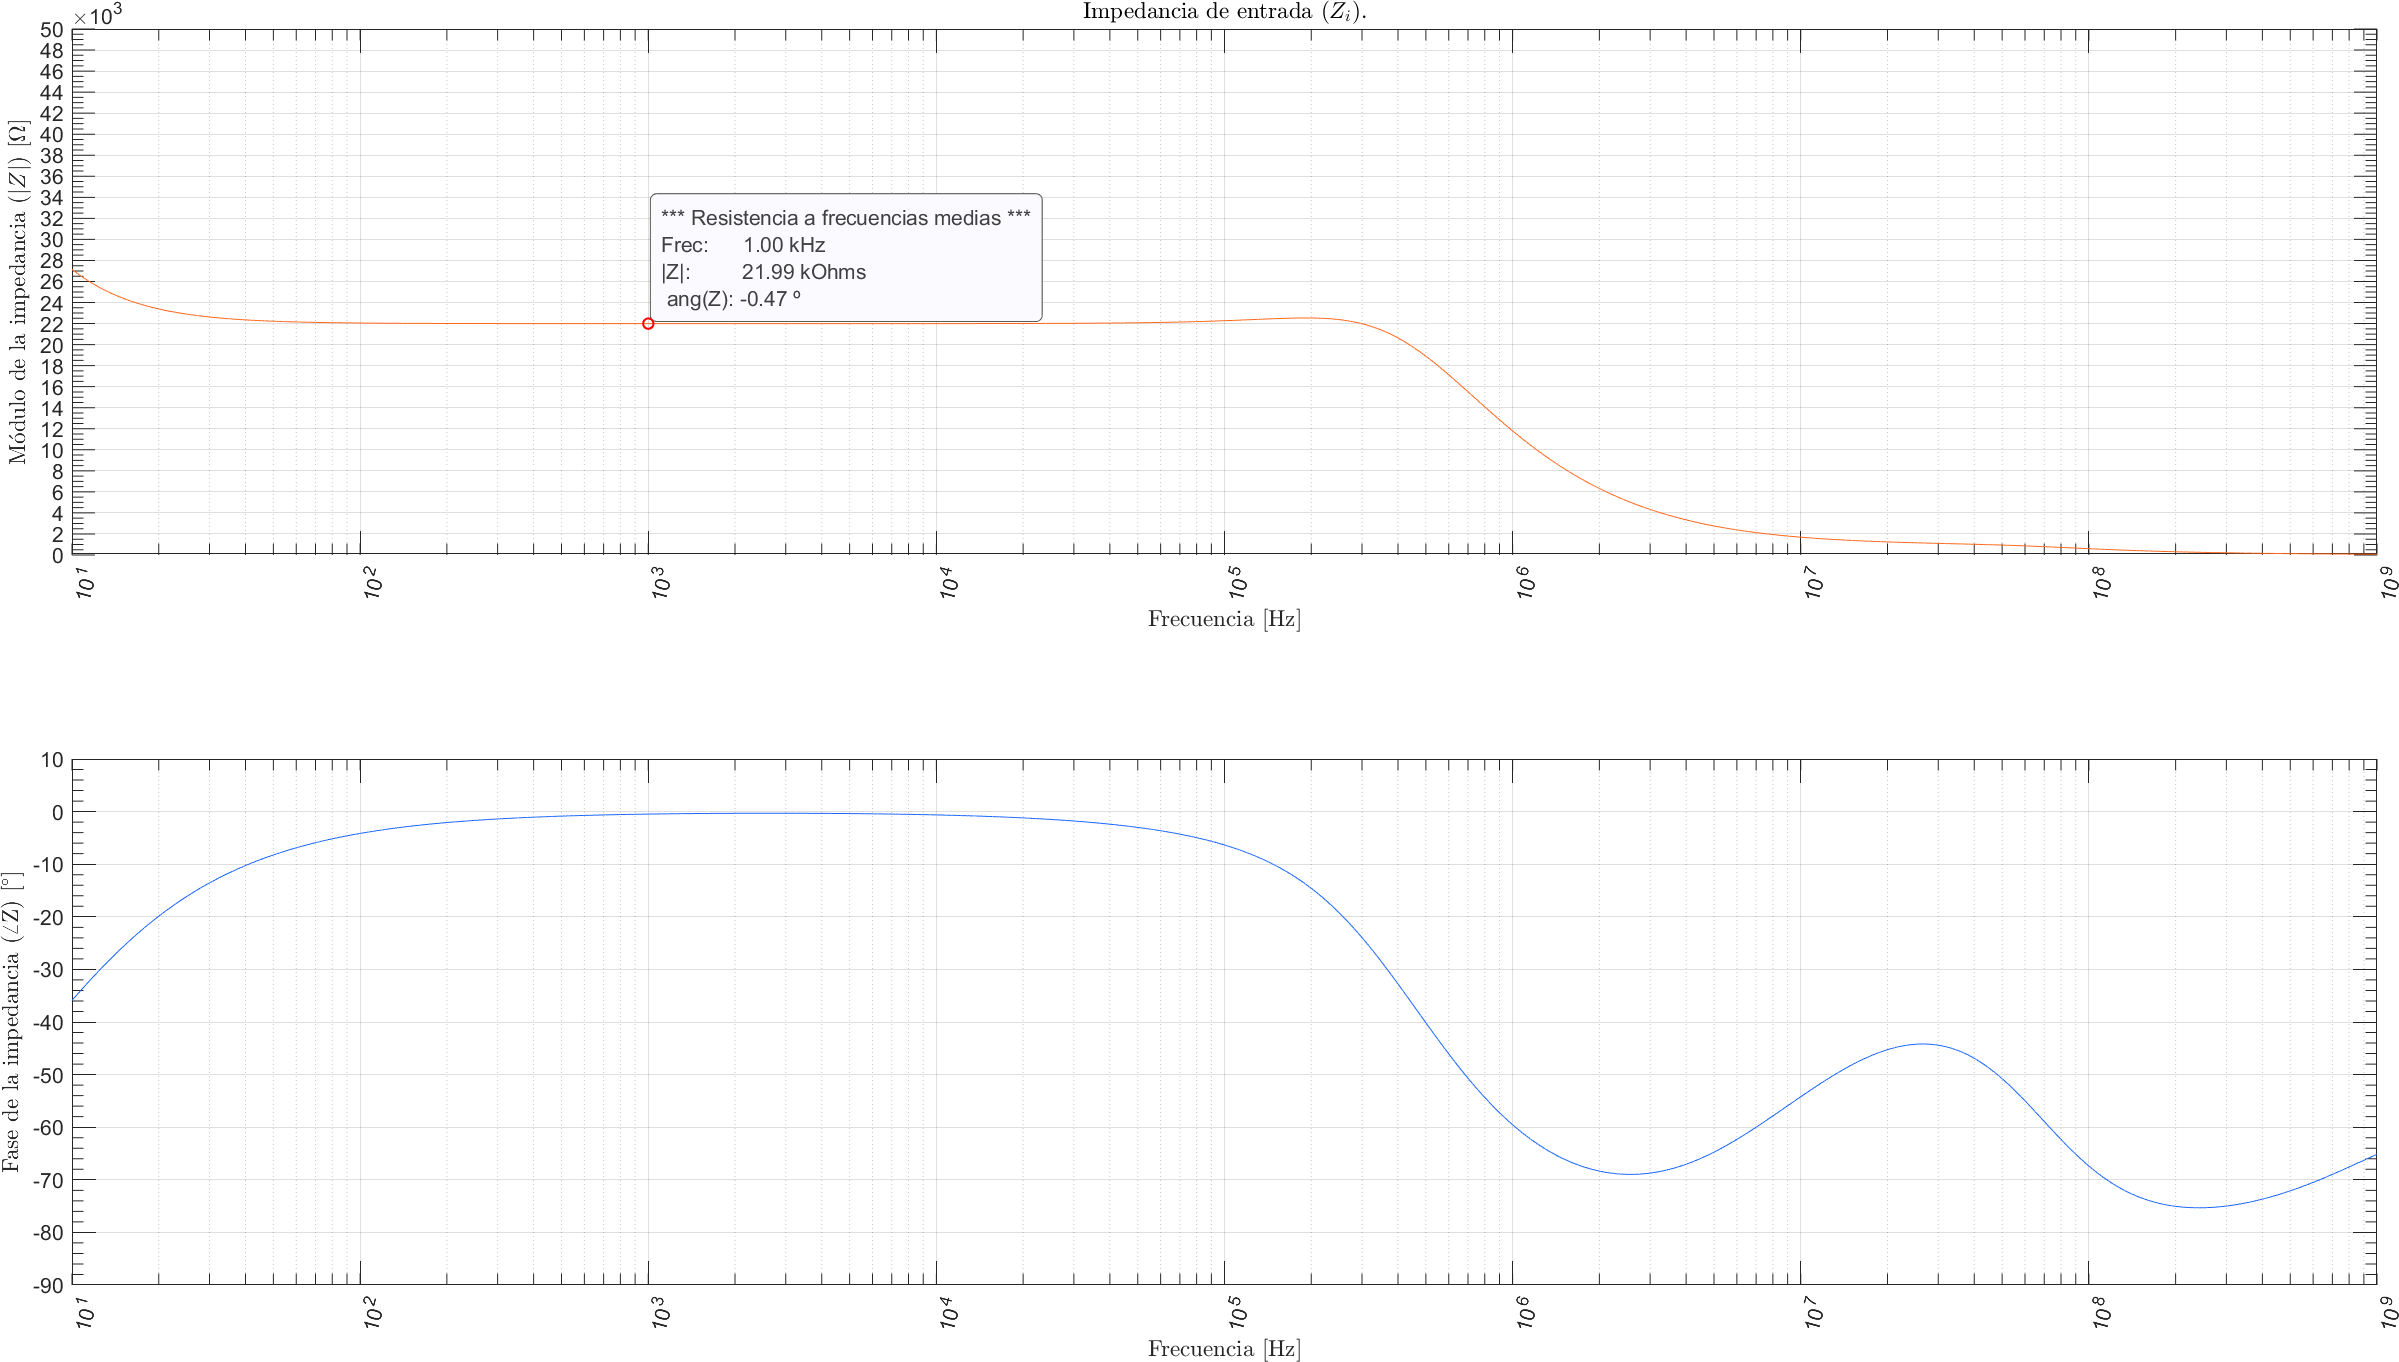
\includegraphics[scale=0.4]{./img/simulaciones/Impedance/amplifier_Zi.png}
    \caption{Valores de impedancia de entrada mediante simulación}
    \label{fig:amplifier_Zi_sim}
\end{figure}

\begin{figure}[H]
    \centering
    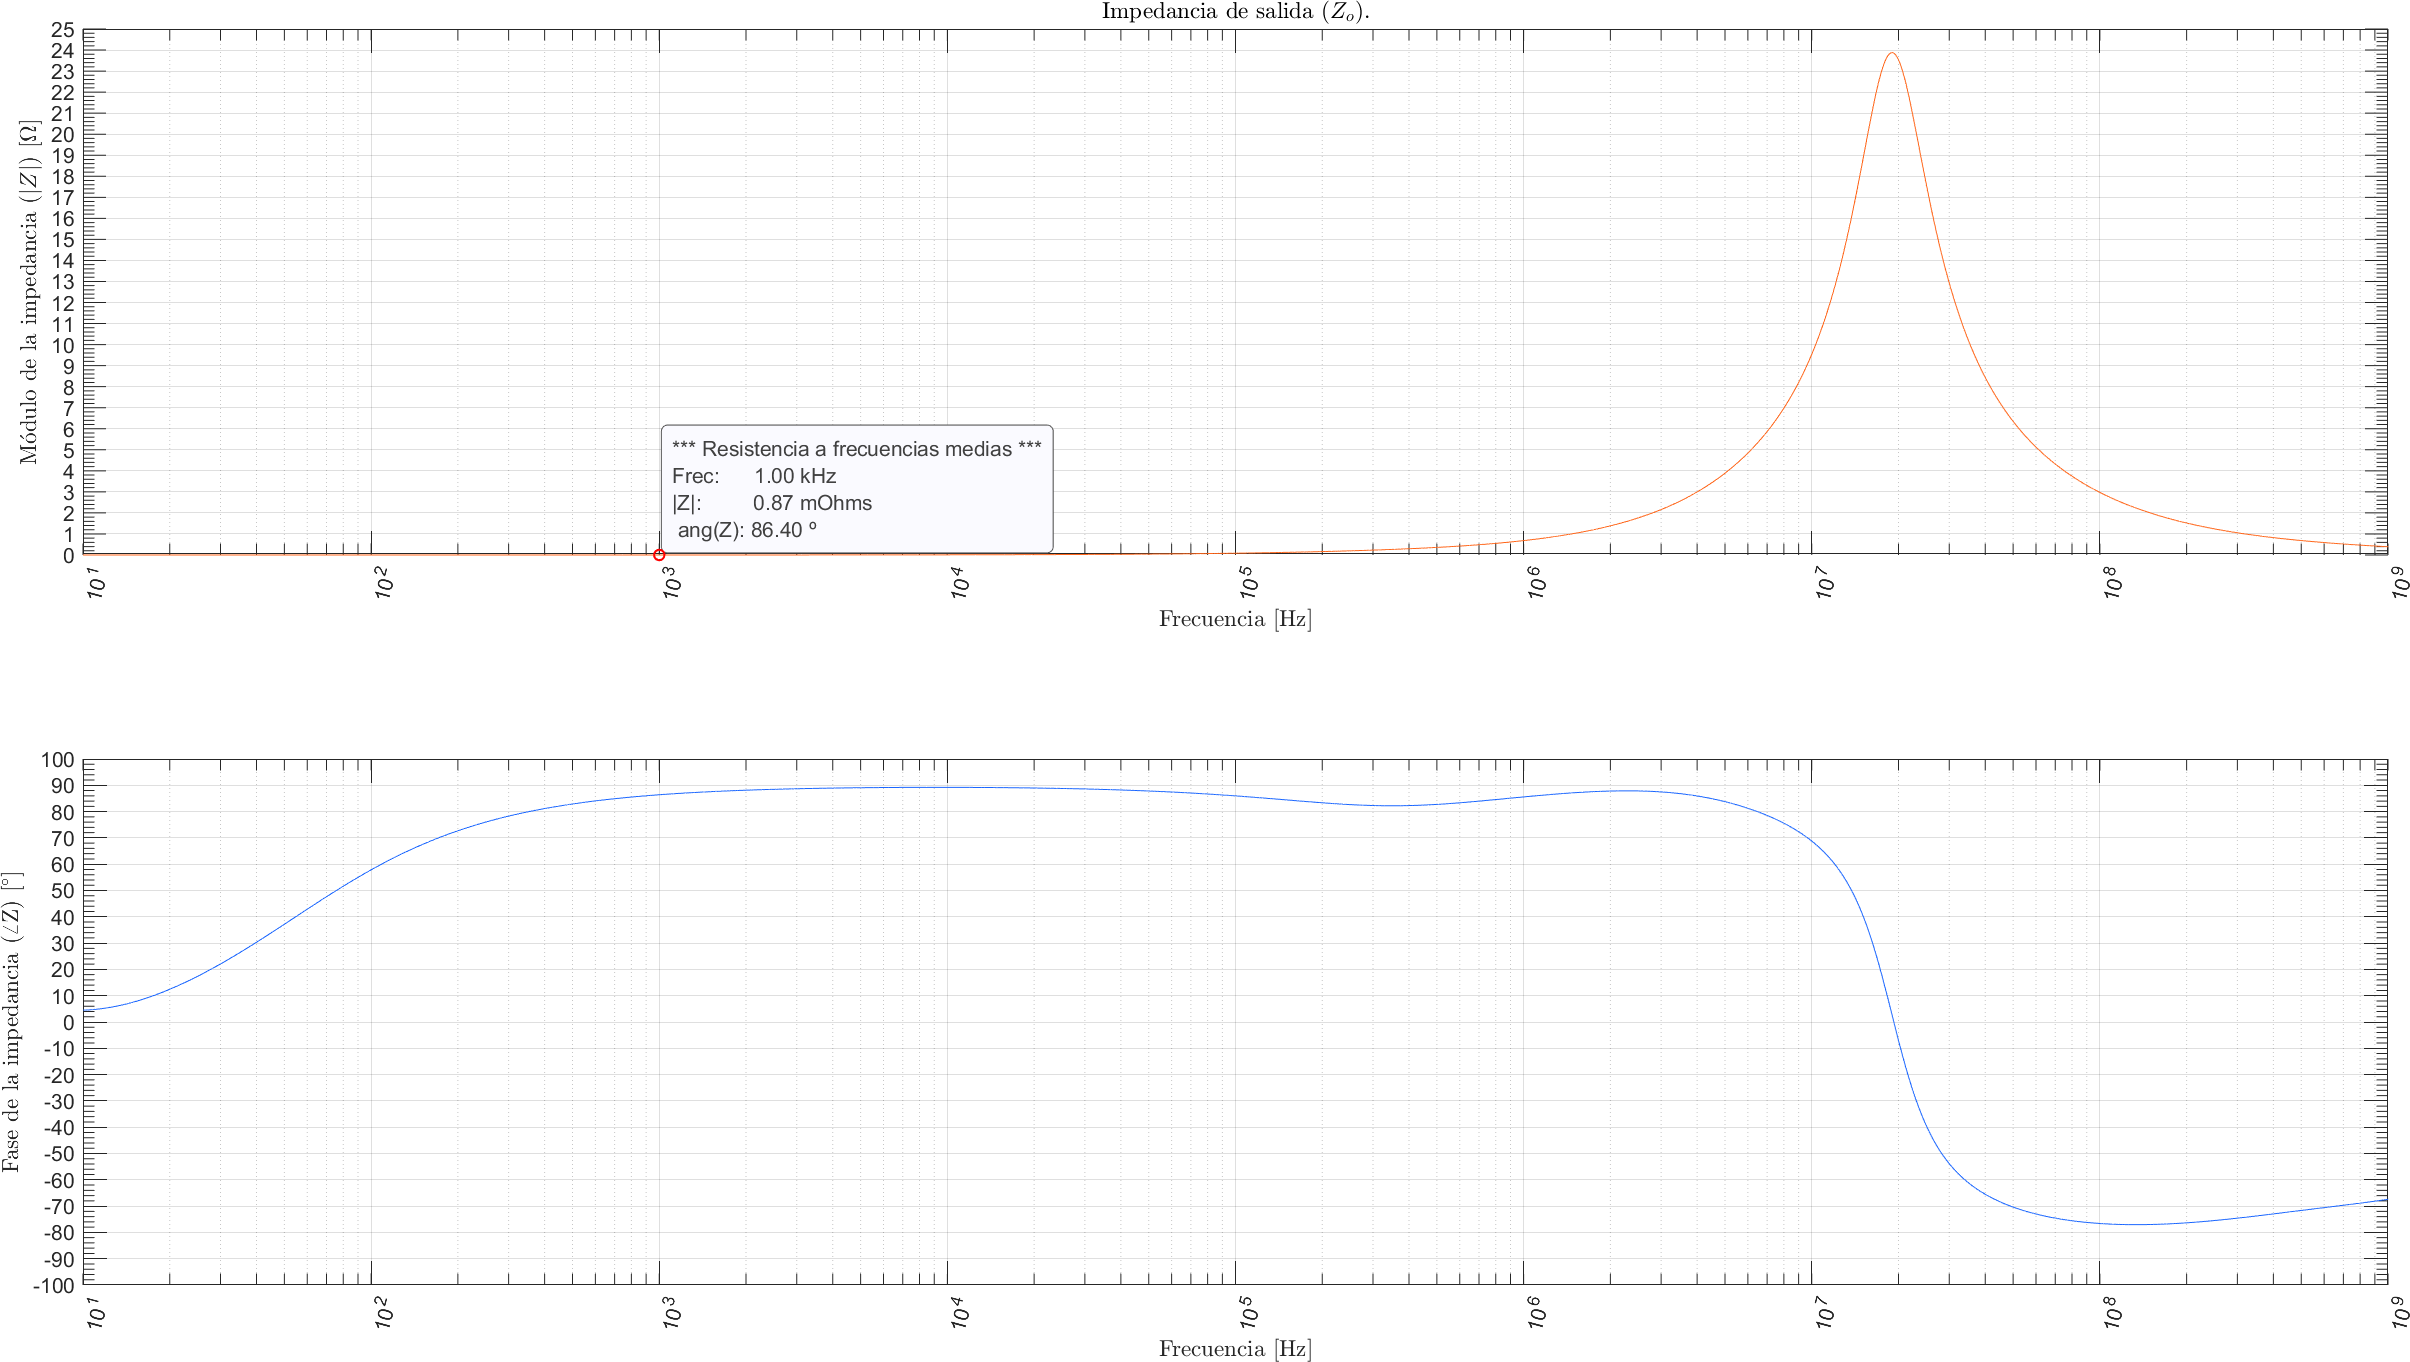
\includegraphics[scale=0.4]{./img/simulaciones/Impedance/amplifier_Zo.png}
    \caption{Valores de impedancia de salida mediante simulación}
    \label{fig:amplifier_Zo_sim}
\end{figure}

\subsection{THD}

\begin{figure}[H]
    \centering
    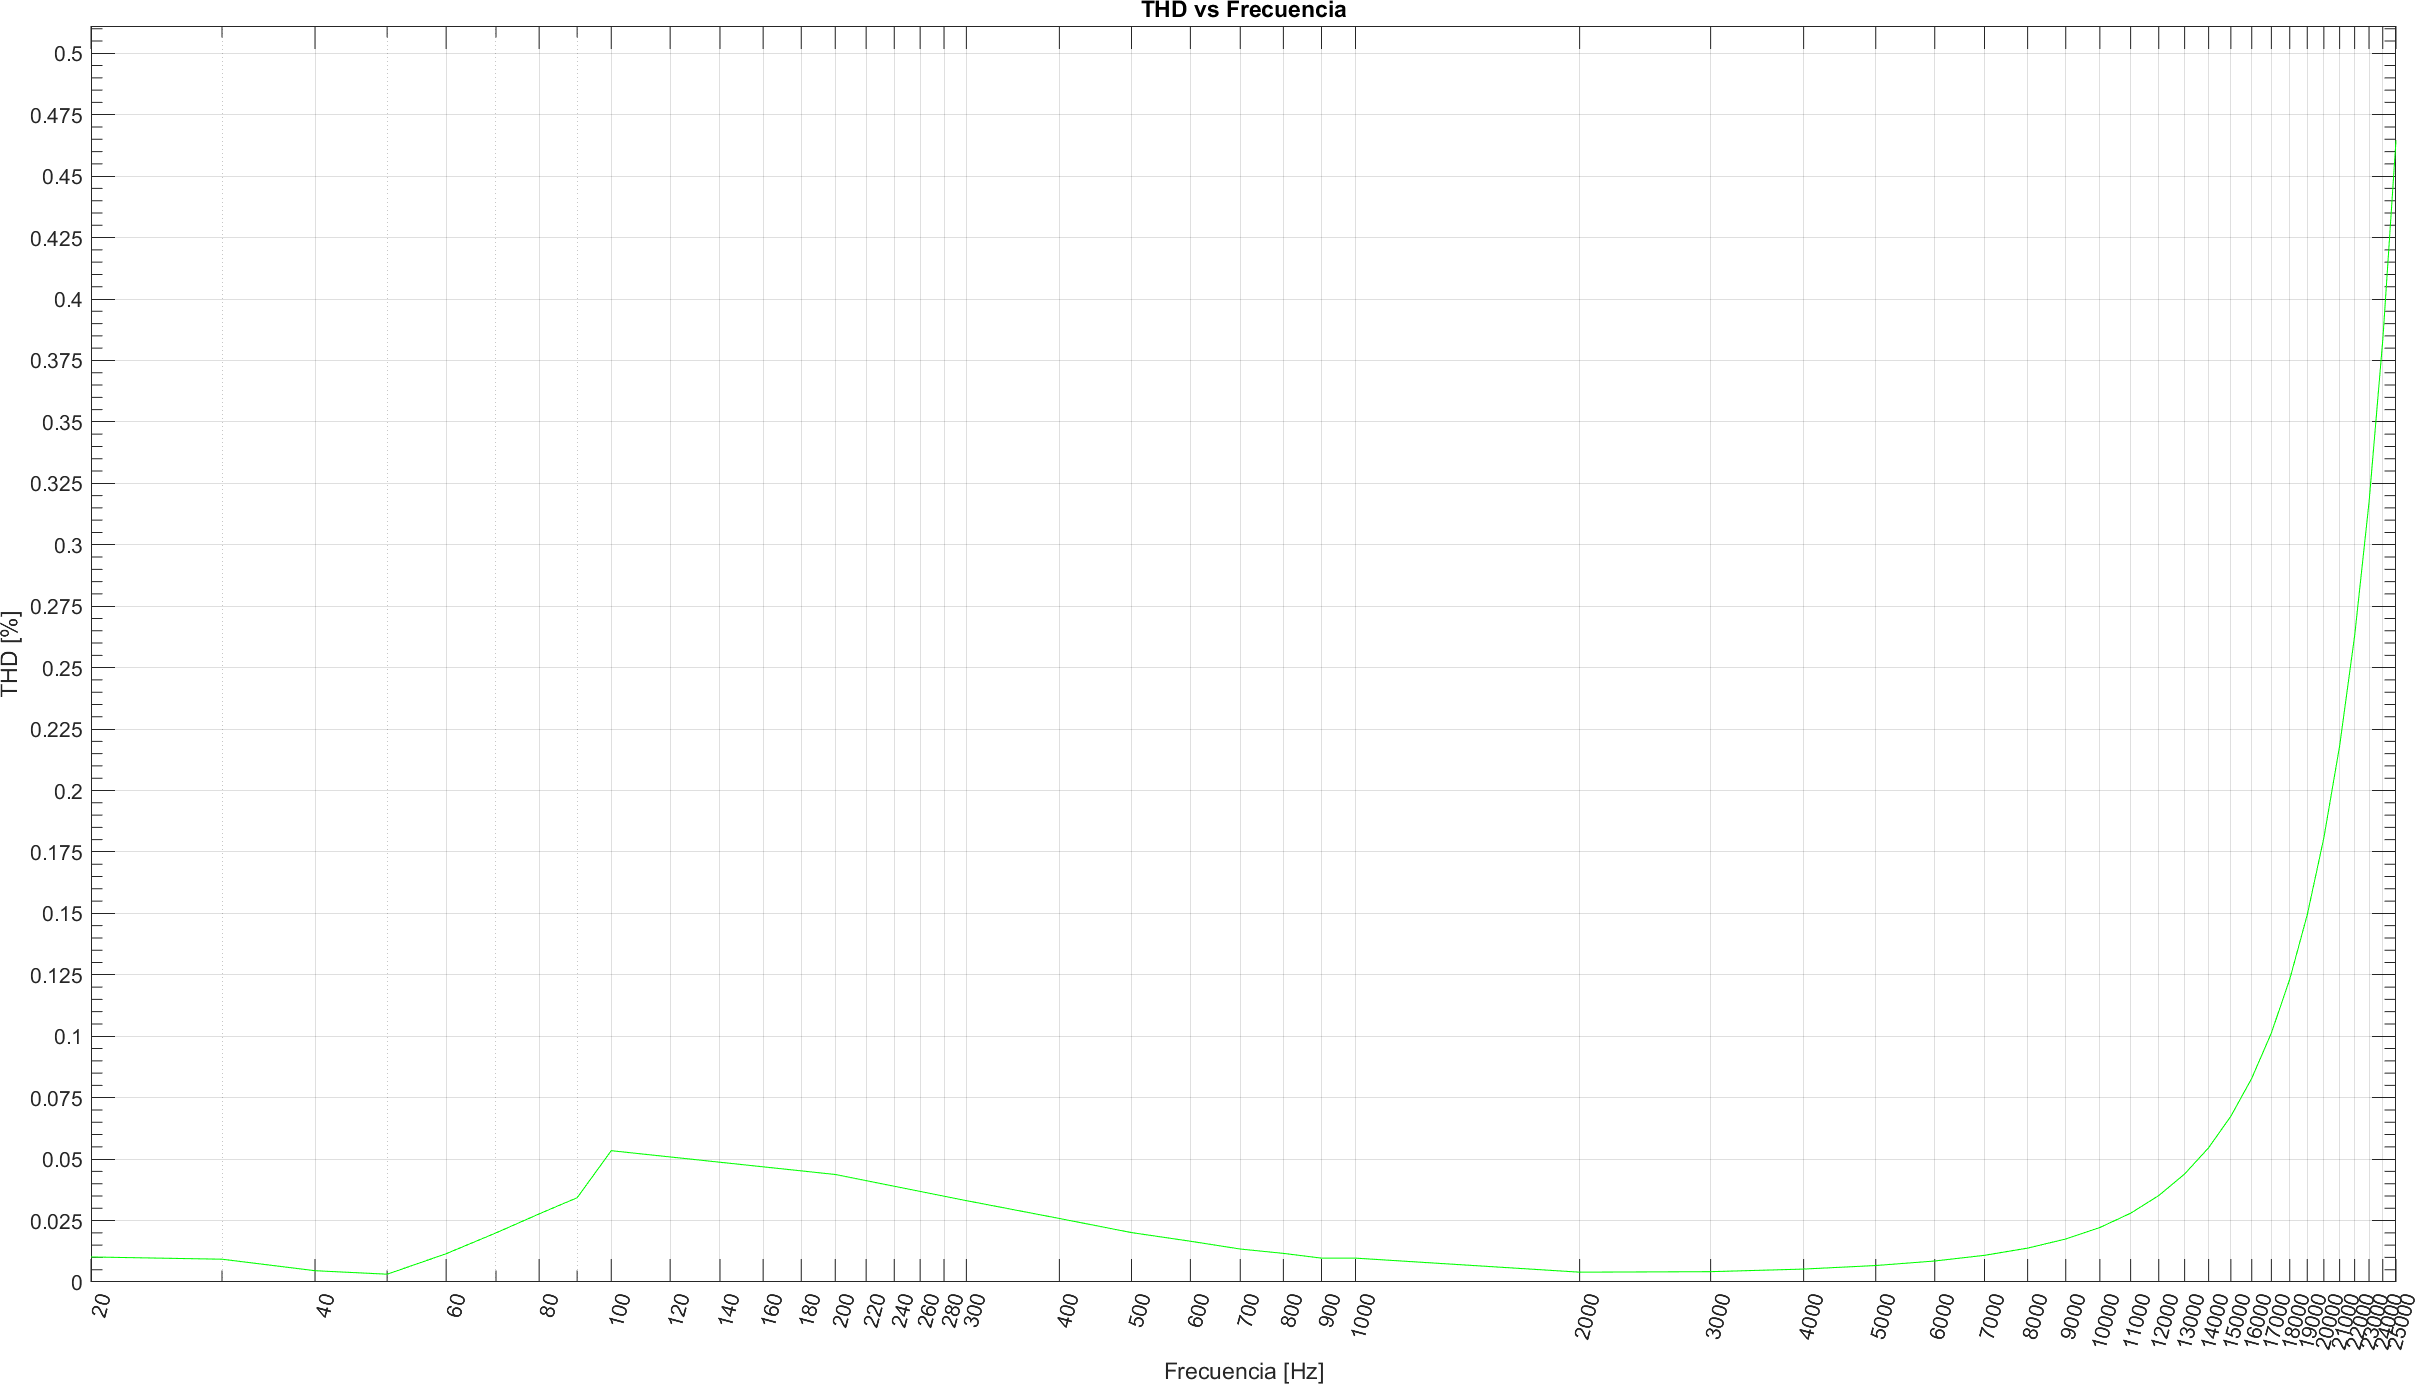
\includegraphics[scale=0.4]{./img/simulaciones/THD/THD_vs_frequency_sim.png}
    \caption{THD en función de la frecuencia según la simulación}
    \label{fig:THD_vs_frequency_sim}
\end{figure}

\begin{figure}[H]
    \centering
    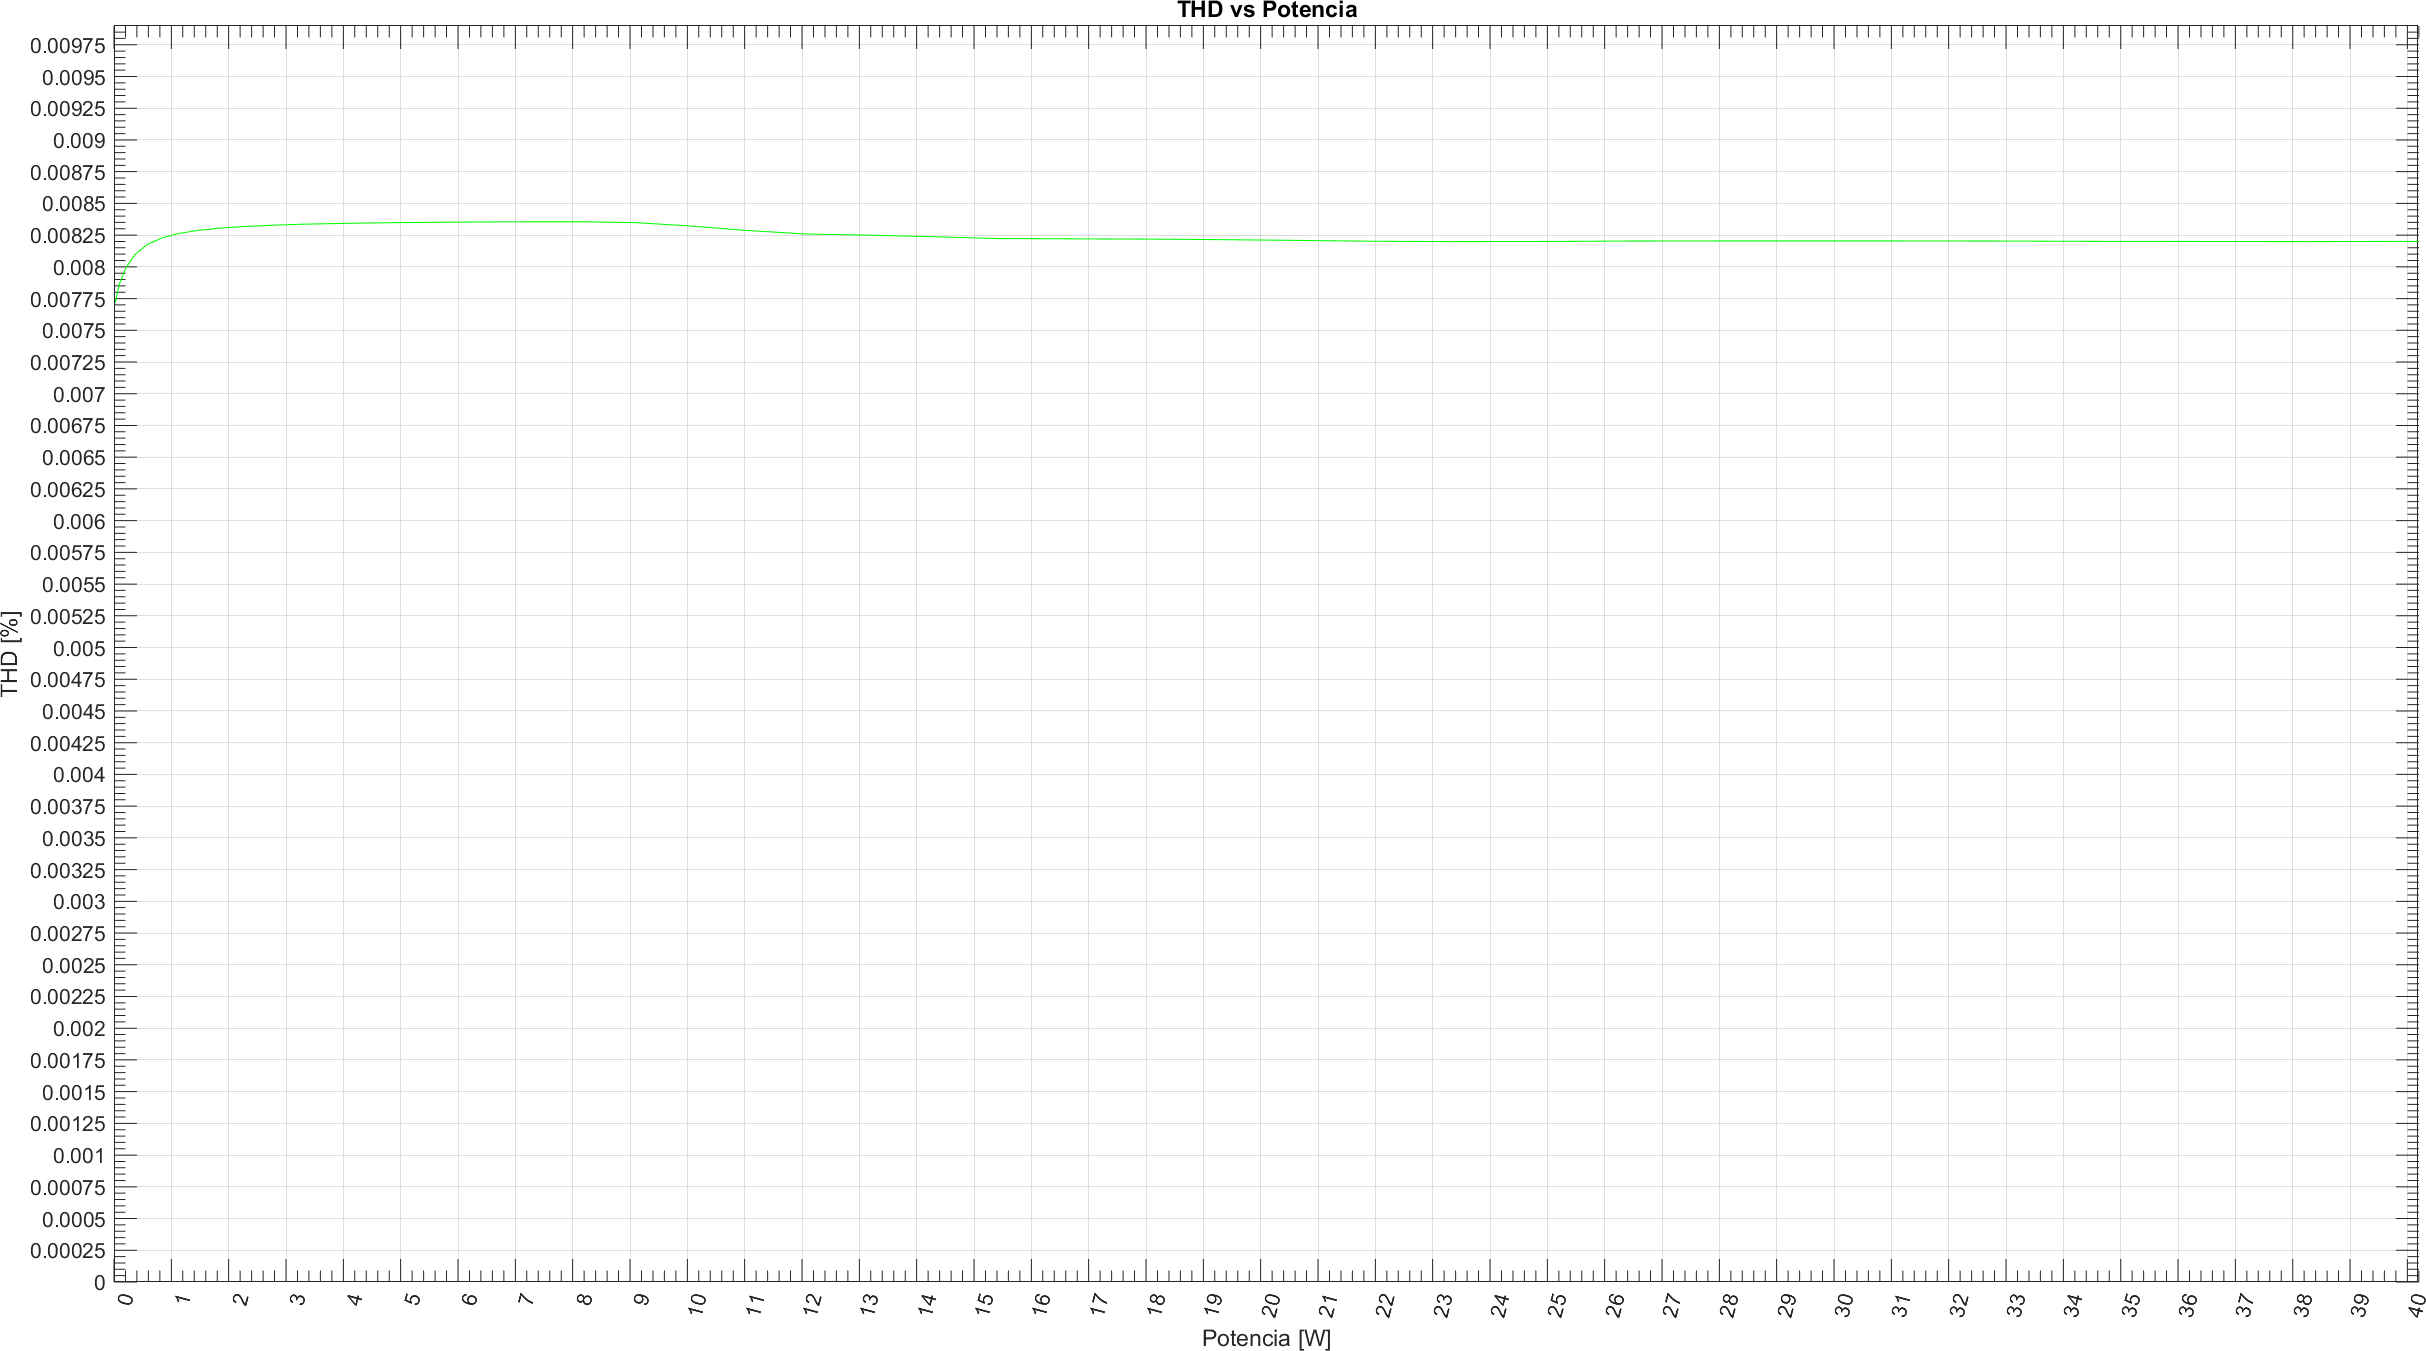
\includegraphics[scale=0.4]{./img/simulaciones/THD/THD_vs_power_sim.png}
    \caption{THD en función de la potencia según la simulación}
    \label{fig:THD_vs_power_sim}
\end{figure}